% !TEX root = ../Thesis.tex

\chapter{Literature Review}
\label{chap:litRev}

Having introduced the background theory to the work discussed in this report, I turn to a more detailed examination of the literature surrounding this work.
I begin with the various relaxation and decoherence processes for spins bound to donors in silicon.
First discussing the mechanisms by which these processes occur I shall then move on to the effect of illumination on these mechanisms.
Following this I shall move on the the stark shift of donor spins in silicon, including a brief introduction to the principle before an examination of previous work performed to characterise this effect in the various species of donor in silicon.


\section{Mechanisms of Relaxation and Decoherence}

The concept of $T_1, T_2$ and $T_2^*$ time was introduced in section \ref{sec:relProc} as the characteristic relaxation, decoherence and dephasing respectively. 
I shall now focus on the established mechanisms by which these occur, looking mainly at relaxation and decoherence as these represent a permanent loss of information.

\subsection{Relaxation}

The relaxation time, $T_1$, determines the rate at which the polarisation of an ensemble of spins returns to Boltzmann equilibrium after being disturbed.
The first method of relaxation that should be considered is spontaneous emission: the emission of a photon into free space as the spin relaxes from excited to ground state. 
For a magnetic dipole this rate is slow in normal circumstances - thousands of seconds or more \cite{schweiger2001principles,Baranov2017}. 
Given that above millikelvin temperatures the rate of transverse relaxation for donor spins in silicon is significantly greater than this it can be neglected as a dominant mechanism.
\\
Spin-lattice relaxation occurs instead via the interaction with of the spin system with vibrations in the silicon lattice - phonons. 
There are three different phonon-mediated processes that affect the relaxation rate of spin systems with transition frequency $\omega_s$, all of which are well described in a 1961 paper by Orbach \cite{VanVleck1940,Orbach1961}.
\\
\textbf{Direct Process}
\\
\noindent\rule{\columnwidth}{1pt}
\begin{adjustwidth}{1.5cm}{}
The first of these is a \textbf{direct process}, whereby a single phonon with frequency equal to that of the spin transition (as given by equation \ref{eq:spinHam}) is emitted into the lattice. 
This rate ($\propto 1/T_1$) is proportional to the phonon density at $\omega_s$ and varies with spin transition frequency and temperature as: $\omega_s^4T^{-1}$.
\par
\par
\end{adjustwidth}
\textbf{Raman Process}
\par\noindent\rule{\columnwidth}{1pt}
\begin{adjustwidth}{1.5cm}{}
Whilst this rate dominates at lower temperatures, $<10$k, at temperatures with $k_BT \gg \hslash\omega_s$, a two phonon Raman transition becomes more efficient.
As the maximum phonon density is at much higher frequencies than $\omega_s$, the spin first absorbs a phonon at $\omega_{\text{max}}$ before emitting a phonon with $\omega = \omega_{\text{max}} + \omega_s$. 
This corresponds to the spin transitioning to a virtual energy level before rapidly transitioning back to the spin ground state.
For non-integer spin systems the rate due to this effect scales with temperature as: $T^{7}$.
\end{adjustwidth}
\textbf{Orbach Process}
\\
\noindent\rule{\columnwidth}{1pt}
\begin{adjustwidth}{1.5cm}{}
The Raman process involves a virtual energy level so is an inherently off-resonant effect. 
It is possible for the spin to transition to an actual excited state during the two phonon process. 
This is known as an Orbach process and is more efficient than either process above. 
It scales with temperature as: $\exp\left({-\Delta E/K_BT}\right)-1$.
\end{adjustwidth}

\subsection{Decoherence}

At high temperatures the spin-lattice relaxation rate tends to be the dominant process for spins in silicon.
However, at temperatures below $\approx 10$k other factors become limiting. 
In particular the decoherence or $T_2$ time becomes important. 
This is the process by which the spins lose phase coherence irreversibly. 
There are several mechanisms that contribute to $T_2$, detailed here.
\\
\textbf{Spectral Diffusion}
\\
The first of these is spectral diffusion and its impact is largely dependent on the sample used.
In natural silicon samples there is a relatively high concentration of Spin-$\frac{1}{2}$ $^{29}$Si nuclear spins ($4.7\%4$). 
Due to the large extent of the donor electron wavefunction, it is highly probable that a given donor will experience a hyperfine interaction with one or more of these nuclei.
Although the large difference between the electron and nuclear gyromagnetic ratios prevents a state exchange or 'flip-flop' interaction, nearby pairs of $^{29}$Si nuclei do have this interaction.
The rate of exchange is slow, ($\approx 100$Hz) and will cause a change in the hyperfine interaction with any nearby donor electrons.
This will cause the acquisition of phase differences between electrons over time.
As these changes are time dependent they are \textit{not} refocused by a Hahn echo sequence \cite{Wolfowicz2015a}. 
In purified silicon samples this effect is reduced to the point that it is no longer the limiting factor in spin coherence.
\\
\textbf{Instantaneous Diffusion}
\\
In the first experiments on spin coherence times on purified silicon, the increase in coherence time was found to be on the order 2 fold \cite{Gordon1958}.
The reason behind this limited increase was the high donor concentrations, leading to interaction between donors.
Spins close enough to interact with one another will experience slightly different magnetic fields and the random nature of donor distribution leads to this effect being inhomogeneous.
Once again, this will not be reversed by a Hahn echo sequence as two donors interacting with one another will both be flipped, meaning that the phase acquisition is unchanged.
This effect is dependent on the concentration of donors in a sample according to:

\begin{equation}
\frac{1}{T_{2}^{\text{ID}}} = C(2\pi\gamma_e)^2\frac{\pi}{9\sqrt{3}}\mu_0\hslash,
\label{eq:instDiff}
\end{equation}

where C is the donor concentration.
\\
At concentrations useful for ESR techniques and at sufficiently low temperatures instantaneous diffusion will be a limiting factor in spin coherence times in almost all cases.
One technique employed by Tyryshkin \textit{et al}, open to ensemble based approaches such as ESR but not to single qubit control, is to use refocussing pulses of angle $<\pi$ in the Hahn echo sequence \cite{Tyryshkin2011}.
This effectively refocuses fewer spins during the Hahn echo sequence. 
This reduces the signal but increases $T_2$ time as the effect of instantaneous diffusion is suppressed by addressed spins being on average much further apart. 
At this point three further effects become limiting:

\begin{itemize}
\item \textit{Direct $T_1$ Flips}: only relevant at higher temperatures when $T_1$ is close to the intrinsic $T_2$, $>10$k. This is the process of a single donor flipping to its ground state, thereby destroying its coherence.
\item \textit{Spectral Diffusion from donors}: the limiting factor at low temperatures $<4$k, this process is similar to the spectral diffusion for $^{29}$Si spins. Nearby pairs of donors undergo spin exchange, causing any other nearby donors to experience a phase shift as their hyperfine coupling changes. 
\item \textit{$T_1$ of Neighbouring Donors}: this process is important at intermediate temperatures, between $4$k and $10$k. At these temperatures direct $T_1$ flips are yet to dominate but $T_1$ flips of neighbouring donors can affect the magnetic field experienced by a central donor. This effect is known as $T_1$-type spectral diffusion.
This process was identified by Tyryshkin \textit{et al} as producing lower than expected $T_2$ times when $T_1$ appeared to no longer be a limiting factor \cite{Tyryshkin2011}. 
The decoherence rate as a function of $T_1$ induced spectral diffusion has a characteristic, stretched exponential of the form $\exp(-(2\tau/T_{SD})^2)$, with $T_2^{SD} = \sqrt[]{T_1}$.
\end{itemize}

The five key contributors to decoherence are shown in figure \ref{fig:decoherenceTypes}.
The key contributors to decoherence times are then:

\begin{itemize}
\item \textit{Temperature}: when $T_1$ is sufficiently short at high temperatures the $T_1$ of the donors will restrict $T_2$. At intermediate temperatures $T_1$ flips of neighbouring donors induces spectral diffusion, reducing $T_2$.
\item \textit{Sample Purity}: the concentration of $^{29}$Si spins in the silicon has a significant impact on $T_2$ due to spectral diffusion via nuclear spin flip-flop.
\item \textit{Donor Concentration}: the concentration of donors increases the rate of instantaneous diffusion, indirect flip-flop, direct flip-flop and $T_1$ type spectral diffusion. 
\end{itemize}

With the mechanisms of decoherence addressed, we now turn to examine the effect of illumination on donor relaxation and coherence rates.

\begin{figure}
\centering
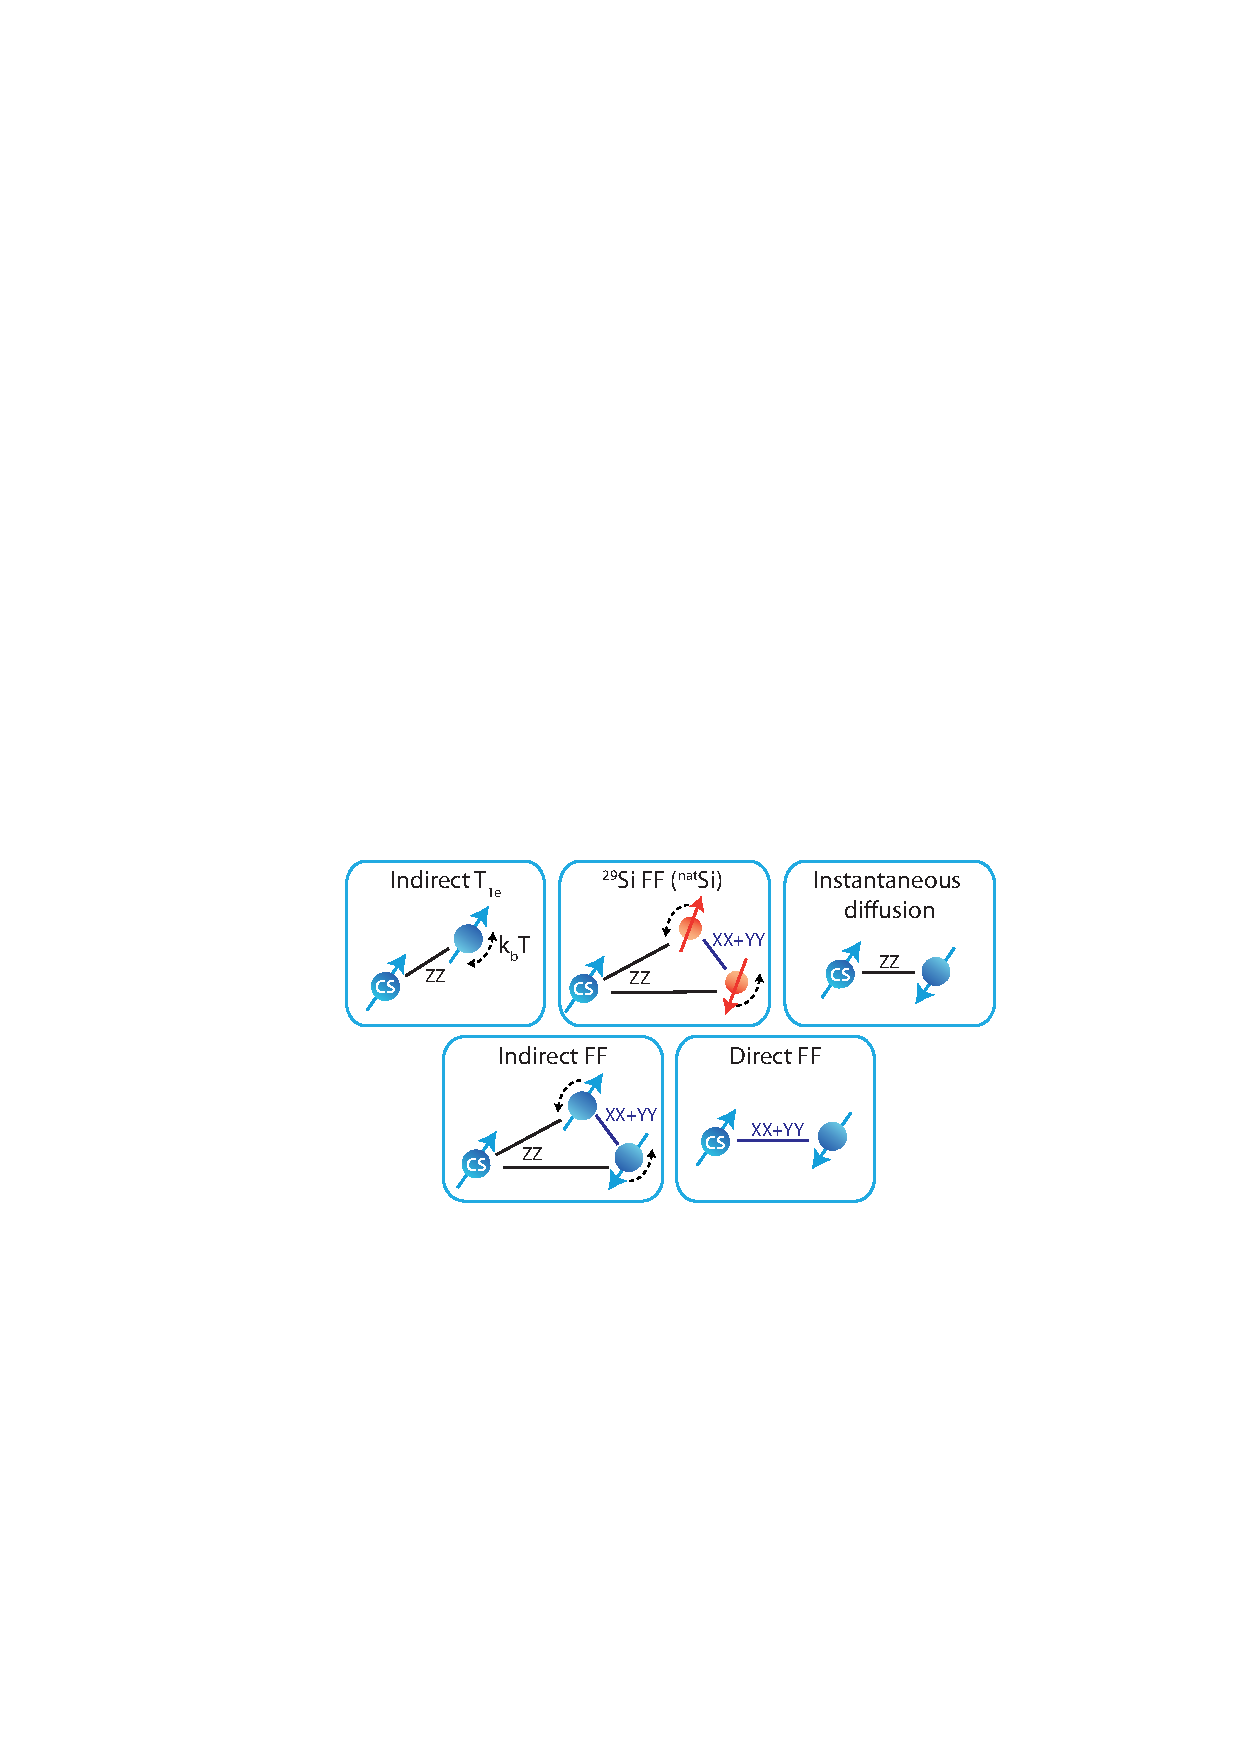
\includegraphics[width = \columnwidth]{Figures/decoherenceTypes.pdf}
\caption[Decoherence mechanisms in silicon]{Cartoon showing the five key types of decoherence mechanisms for donor electrons in silicon. Indirect $T_1$ is the relaxation of a neighbouring donor modulating the magnetic field at a central donor. Flip-flops of $^{29}$Si nuclear pairs modulating the magnetic field at the donor. Instantaneous diffusion is the inhomogeneous phase acquisition of donors due to different inter-donor spacings. Indirect flip-flop mechanism is similar to that involving $^{29}$Si nuclei but with pairs of donors. Direct flip-flop is state exchange between a central donor and a neighbour. Figure is taken from \cite{Wolfowicz2015a}.}
\label{fig:decoherenceTypes}
\end{figure}



\section{Illumination and Decoherence}

\subsection{Free Carriers and Decoherence}

The discussion above centred on the typical factors that affect coherence and relaxation times:  temperature, donor concentration and silicon purity.
One of the key questions addressed in this report is the impact of another factor on relaxation times: illumination.
Feher and Gere were among the first to examine this impact in their 1959 paper \cite{Gere1959}, analysed using CW ESR of phosphorus donors in silicon. 
The key question that they examined is the impact of illumination wavelength on relaxation time, the results of which can be seen in figure \ref{fig:phosPhotFeher}. 
The important result here is the sharp increase in relaxation rate as the photon energies exceed that of the silicon band gap, $\approx 1.12$eV.
As this energy is exceeded by the photons, free carriers are created in the silicon conduction band as electrons are promoted from the valence band.
These free carriers can scatter off the electrons bound to the phosphorus donors, causing them to relax via a state exchange.
Feher and Gere postulate two possible processes that could cause this relaxation: the first is direct scattering of a donor electron by a free electron, whilst the second is a two stage process.
They identify the second of these as dominant, due in the main to the low number of free electrons relative to donors in their experiments - $5\times10^6$ vs $7\times10^{15}$ - with each interaction requiring the subsequent relaxation of the conduction electron to the lattice.
The double spin exchange process does not involve the free electron changing spin, instead both the nuclear spin of the donor and the electron bound to it change spin state. 
This removes the requirement that the conduction electron subsequently relax to the valence band, significantly increasing the rate of the process.
\\

\begin{figure}
\centering
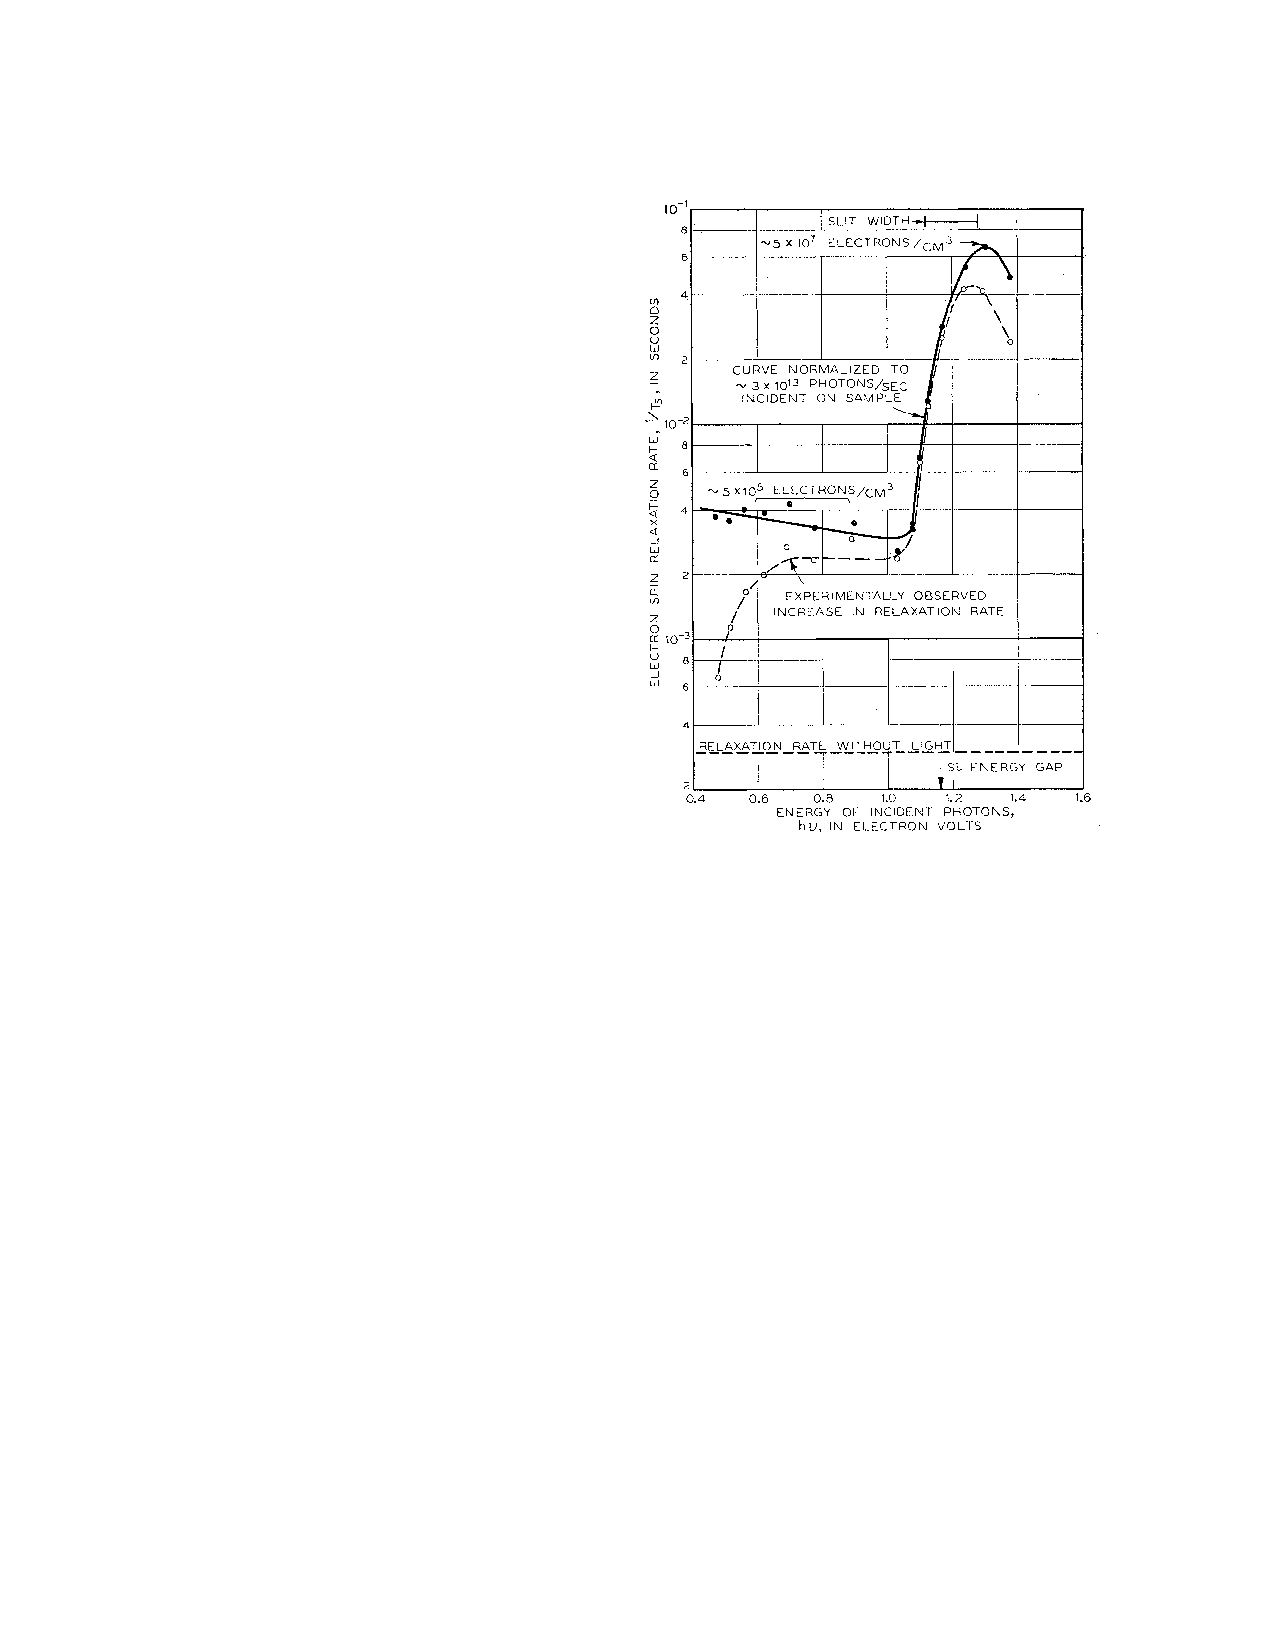
\includegraphics[width = 0.75\columnwidth]{Figures/photEngDep.pdf}
\caption[$T_1$ dependence on photon energy]{Graph from \cite{Gere1959} showing the measured dependence of relaxation time on photon energy. Notable is the sharp increase in relaxation rate for photon energies in excess of 1.10eV. The main cause of this is that this is the energy of the photon band gap, meaning that free electrons are created in the silicon conduction band. These free electrons can then scatter off the electrons bound to donors in silicon, causing them to relax.}
\label{fig:phosPhotFeher}
\end{figure}

The work done by Feher and Gere was performed using only CW ESR, because of this their work addresses only the impact of laser illumination on $T_1$. 
The key timescale for quantum computing is the coherence time, $T_2$, which must be examined using pulsed ESR.
Whilst $T_2$ time will ultimately be limited by $T_1$ a concern is that free carriers in the silicon conduction band will have an impact beyond this.
It seems obvious that the presence of these free carriers could alter the magnetic environment of the donors in a time-dependent and inhomogeneous fashion, potentially having a drastic impact on the coherence time of donors.
Examining the impact of illumination on decoherence times will be an important goal of this report.

\subsubsection{Free Carrier Lifetimes}

One question that is of importance is the time that free carriers will persist for following a laser pulse, as this will determine how long their effects influence relaxation and coherence times.

\subsection{Heating and Decoherence}

A potential factor not addressed by Feher and Gere is the potential impact that heating could have on relaxation and by extension coherence times. 
Although the number of free carriers produced by laser illumination will be significantly reduced as photon energies drop below the band gap, it is possible that heating could still have a significant impact.
Of particular note is the reduced heat capacity of silicon at low temperatures. 
At room temperature heat capacity ($C_p^o$) is 19.1 J.mol$^{-1}$k$^{-1}$, but at cryogenic temperatures this is reduced by several orders of magnitude to approximately 0.004 J.mol$^{-1}$k$^{-1}$ at 8k \cite{Desai1986,Niinikoski1986}.
Clearly then the potential impact of infra-red illumination is obvious - only a small conversion of incident photons to phonons in the lattice could potentially have a significant impact on the relaxation rates for donor spins.
Exploring this potential impact will be a central goal of this report.
\\
Having looked at some of the literature surrounding the questions of relaxation and decoherence of donors in silicon, I now move on to the stark shift of donors in silicon.

\section{The Stark Shift}

\subsection{Introduction}

The Stark shift, at its simplest, is the modulation of the hyperfine coupling between electron and nuclear spins via electric fields.
The Stark shift was employed in Kane's original proposal as a means to control which qubits interact with an applied control pulse \cite{Kane1998}.
As well as the potential application for control of donor spins, the Stark shift presents a problem in the potential for electric field noise to cause decoherence of donor spins.
This impact may become particularly important for single donors close to electrical contacts where distances are short and so fields high.
Clearly then an understanding of the stark shift and its impact on donors is useful both from control and decoherence perspectives.
\\
An intuitive understanding of the stark shift is easily grasped: the electron's wavefunction extends over space and is concentrated at the donor nucleus. 
This concentration determines the hyperfine coupling of the spin to the donor.
An electric field changes this wavefunction, effectively pulling it off the nucleus and changing the hyperfine coupling, as seen in figure \ref{fig:starkShift}.
This in turn changes the energy difference between the two spin states of the electron and modulates its precession frequency in a static magnetic field.

\begin{figure}
\centering
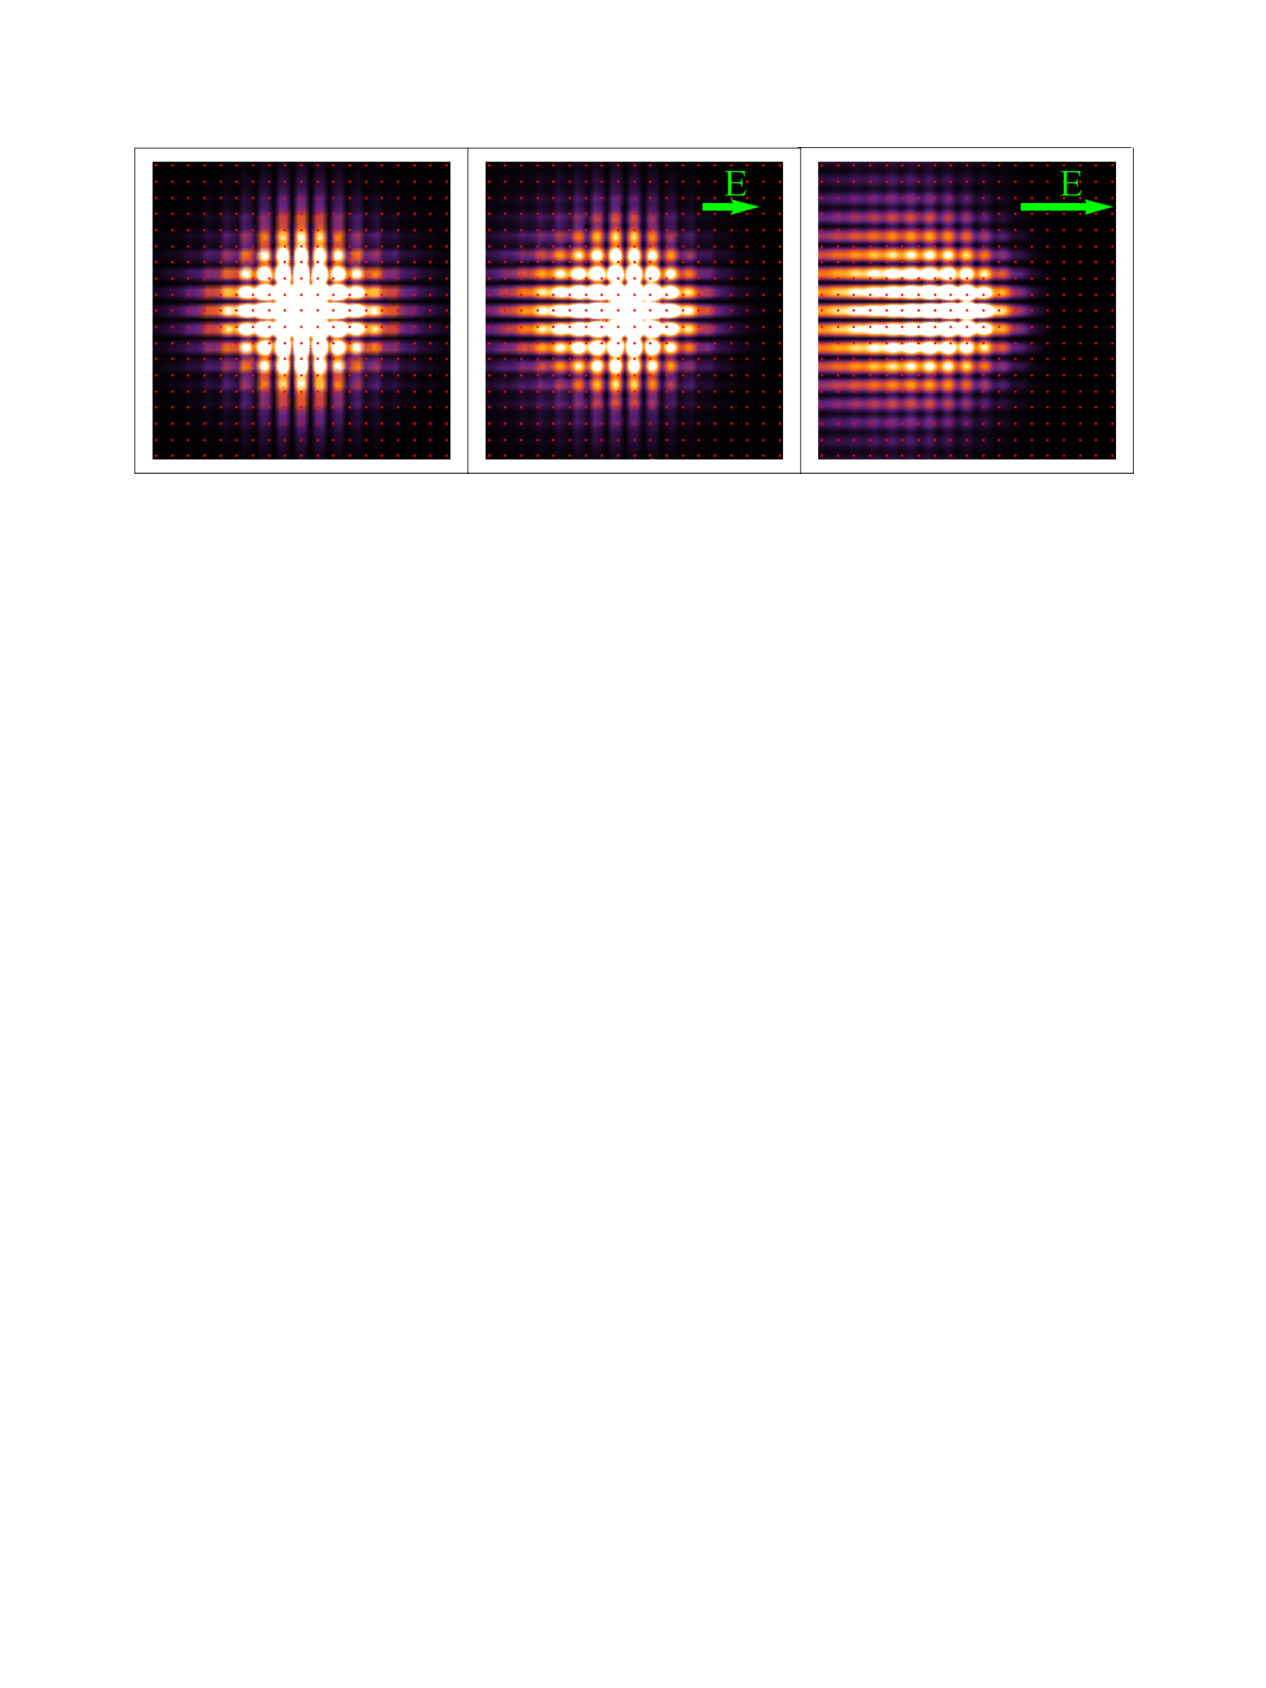
\includegraphics[width=\textwidth]{Figures/starkShift.pdf}
\caption[Electron wavefunction Stark shift]{Simulation showing the density of the electron wavefunction around a donor atom. Red dots represent lattice sites. As an electric field is applied the electron wavefunction is pulled off the central site, changing the strength of its interaction with the donor nucleus and therefore its hyperfine coupling. This shifts the frequency of the electron's spin transition and its precession rate in the magnetic field. Figure reproduced from \cite{Pica2014}.}
\label{fig:starkShift}
\end{figure}

\subsection{Theory}

A technical description of the Stark shift in most cases employs effective mass theory \cite{Pica2014}.
This treats the donor system as if it were a hydrogen atom with a different mass embedded in a silicon lattice as opposed to a vacuum.
This is done by replacing the electron's vacuum mass with its effective mass in the silicon and modifying the vacuum permittivity with the dielectric constant of silicon \cite{Wolfowicz2015a}.
The conduction band of silicon has 6 minima - usually termed 'valleys' - situated in the $\pm x, \pm y, \pm z$ directions and close to the edge of the Brillouin zone, as seen in figure \ref{fig:siliconband}. 

\begin{figure}
\centering
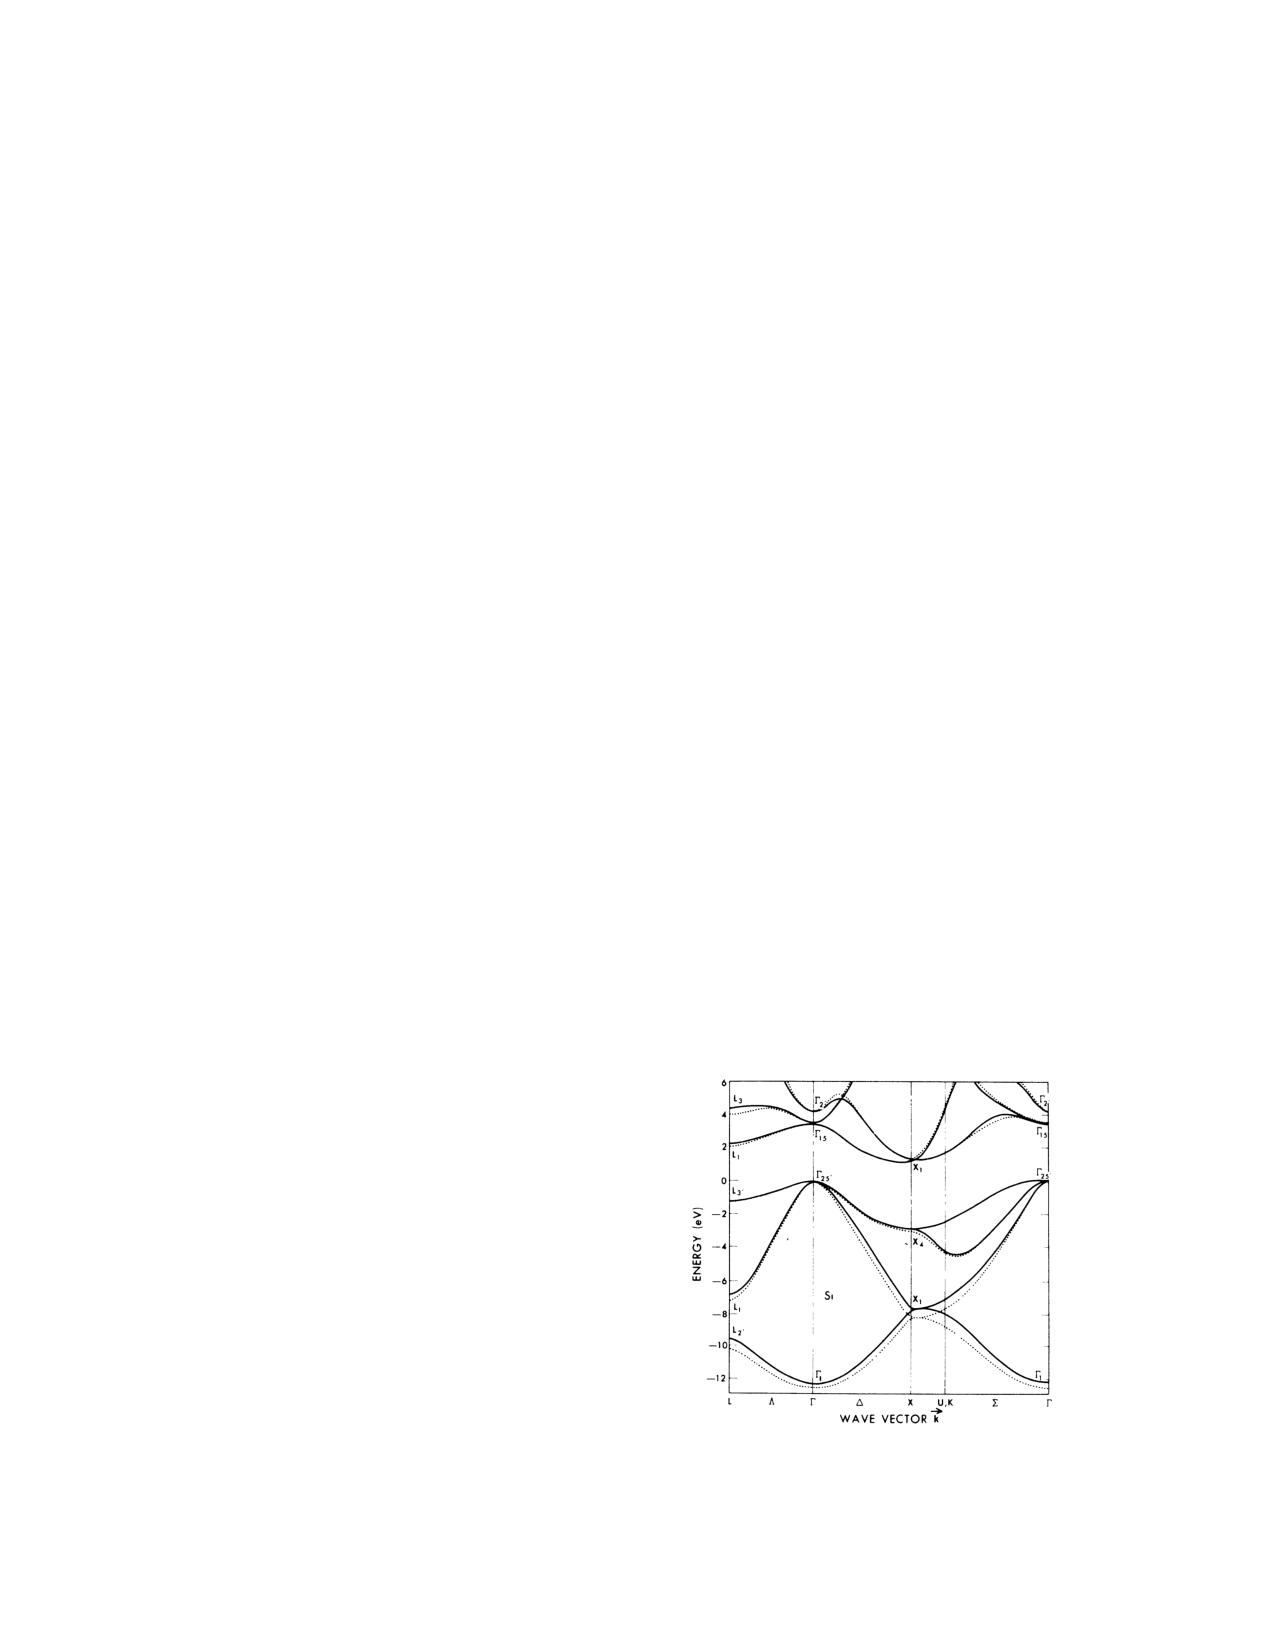
\includegraphics[width = 0.75\columnwidth]{Figures/siliconBandStructure.pdf}
\caption[Silicon band structure]{Figure from \cite{Chelikowsky1974}, showing the band structure of silicon. The top of the valence band is at $\Gamma$, the centre of the Brillouin zone, whilst the minimum of the conduction band is at $X$, towards the edge of the zone.}
\label{fig:siliconband}
\end{figure}

The approach of effective mass theory is to decompose the electron wavefunction into six along these conduction band valleys, giving the equation:

\begin{equation}
\psi(r) = \sum_{\text{i}=1}^6{\alpha_\text{i}\phi_\text{i}(r)F_\text{i}(r)},
\end{equation}

here $\phi_\text{i}(r) = u_\text{i} e^{i \bm{k_\text{i}.r}}$, the Bloch wavefunction such that $u_i(r)$ has the periodicity of the lattice and $\bm{k_\text{i}}=k_0\bm{\text{i}}$ with $k_0$ the momentum value at the valley minimum. 
In the electron ground state these valleys are six-fold degenerate, giving the singlet state \cite{Smit2004}:

\begin{equation}
\text{Singlet  } (1sA_{1}) \text{  }
\begin{cases}
\bm{\alpha_g} = \frac{1}{\sqrt{6}}(1, 1, 1, 1, 1, 1)
\end{cases}
\end{equation}

This ground state is the only state with a component of the electron wavefunction at the nucleus and therefore the only one that experiences a hyperfine coupling. 
The excited states are as follows:

\begin{equation}
\text{Doublet  } (1sE) \text{  }
\begin{cases}
\bm{\alpha_r} = \frac{1}{\sqrt{12}}(-1, -1, -1, -1, 2, 2)\\
\bm{\alpha_s} = \frac{1}{2}(1, 1, -1, -1, 0, 0)\\
\end{cases}
\newline
\text{Triplet  } (1sT_2) \text{  } 
\begin{cases}
\bm{\alpha_x} = \frac{1}{\sqrt{2}}(1, -1, 0, 0, 0, 0)\\
\bm{\alpha_y} = \frac{1}{\sqrt{2}}(0, 0, 1, -1, 0, 0)\\
\bm{\alpha_z} = \frac{1}{\sqrt{12}}(0, 0, 0, 0, 1, -1)\\
\end{cases}
\end{equation}